\documentclass[12pt, letterpaper]{article}
\usepackage{graphicx}
\usepackage{amsmath}
\usepackage{soul}
\usepackage{float}
\usepackage{graphicx}
\graphicspath{ {../graphs/} }


\title{Trimodal analysis}
\author{Brandon Chen}

\begin{document}
\maketitle
\section{Trimodal}

Trimodal: application scans three arrays simultaneously.

\begin{itemize}
\item $x_1$: size of array 1
\item $x_2$: size of array 2
\item $x_3$: size of array 3
\item $p_1$: probability of access array 1
\item $p_2$: probability of access array 2
\item $p_3$: probability of access array 3
\item $d_1 = \frac{x_1}{p_1}$: reuse distance for data in array 1
\item $d_2 = \frac{x_2}{p_2}$: reuse distance for data in array 2
\item $d_3 = \frac{x_3}{p_3}$: reuse distance for data in array 3
\item $ed = p d_1 + p_2 d_2 + p_3 d_3 $: expected reuse distance, equals the
size of working set 
\item S: cache size
\item m: miss rate
\end{itemize}

The reuse distance distribution would look like:
\begin{figure}[H]
\centering
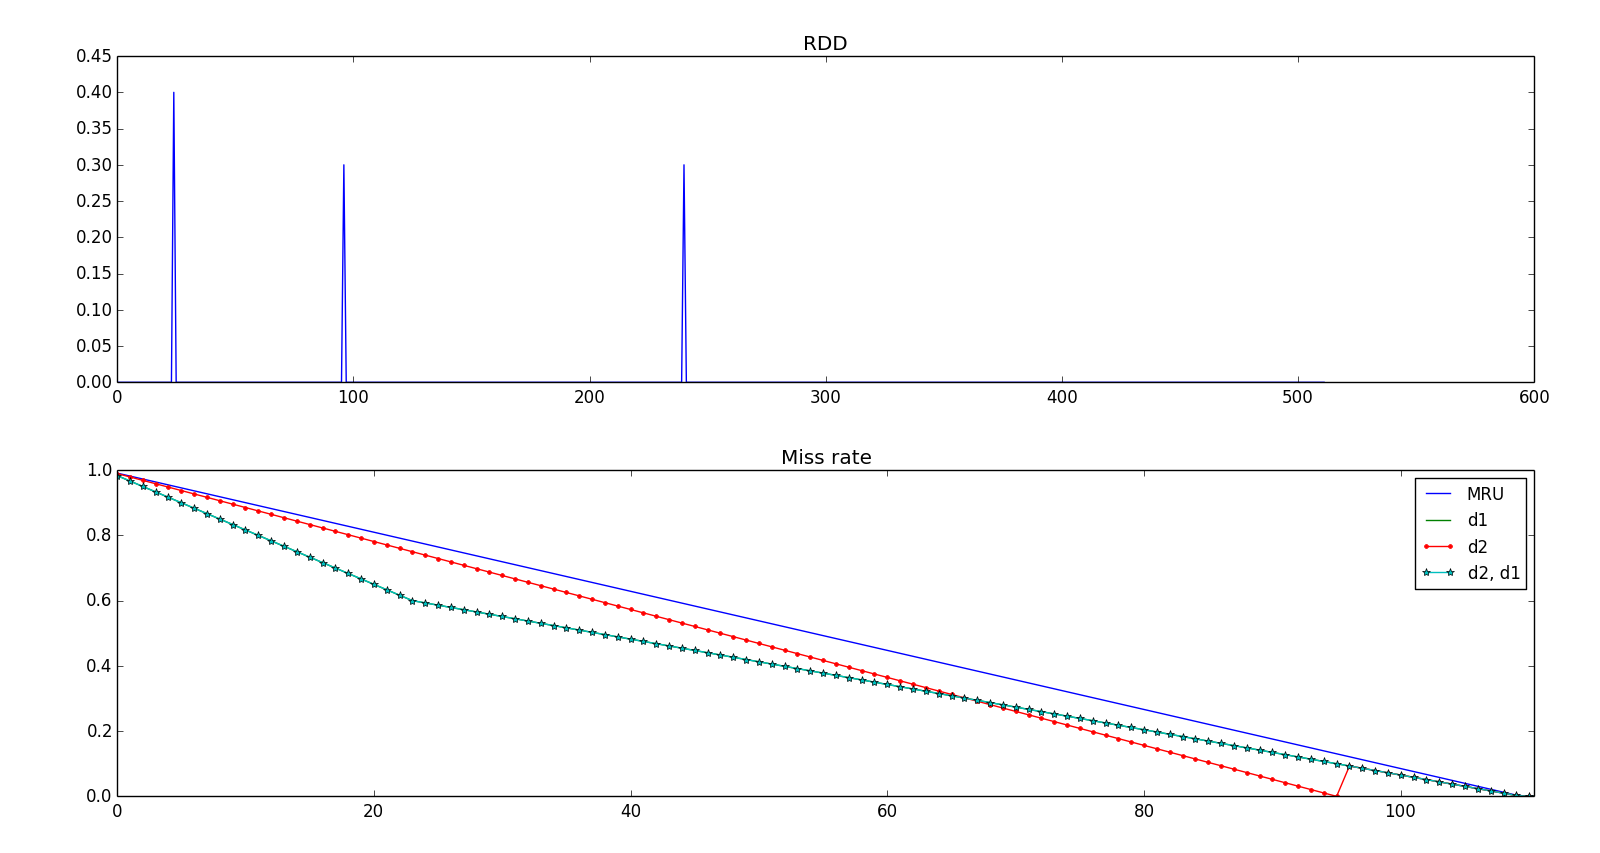
\includegraphics[width=0.5\textwidth]{rdd}
\caption{reuse distance distribution}
\end{figure}

Nathan proposed an awesome cache modeling paper~\cite{beckmann2016modeling}, we
derive the relationship between cache size and miss rate based on the paper's
idea:
\begin{equation}
S = \sum a [H(a) + E(a)]
\end{equation}

This means cache size equals the average lifetime. This may not seem obvious.
Consider every access starts a new lifetime. So the average life time equals to
the expected interval between two consecutive access on the same cache line,
which is S.

\subsection{evict at 0 (MRU)}

\begin{figure}[H]
\centering
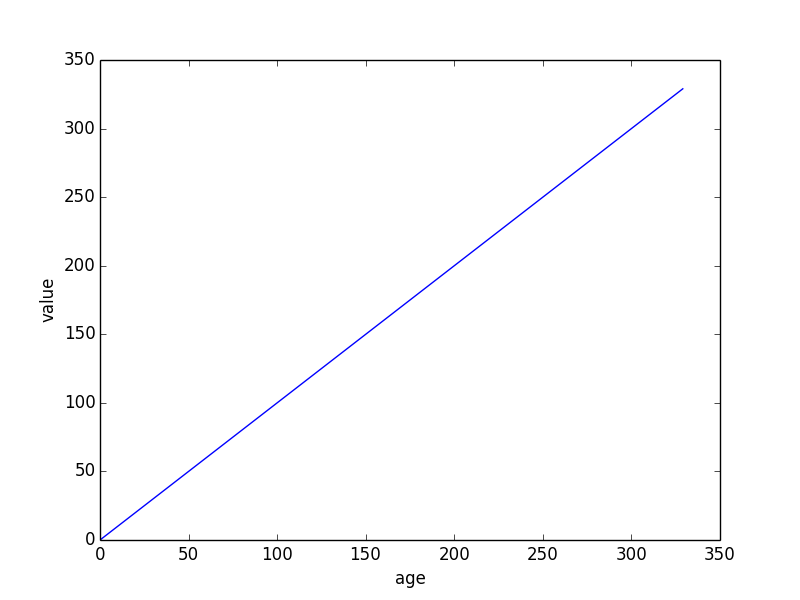
\includegraphics[width=0.5\textwidth]{mru_value}
\caption{policy: mru}
\end{figure}

\begin{table}[H]
\begin{center}
\begin{tabular}{c|c c c c}
\hline
 & 0 & d1 & d2 & d3 \\
 \hline
hit & & $p_1 (1-m)$ & $p_2(1-m)$ & $p_3(1-m)$ \\
evict & m & & & 
\end{tabular}
\caption{events distribution when $0<S<d1$}
\end{center}
\end{table}

\begin{equation}
\begin{aligned}
m = 1 - \frac{S}{ed}
\end{aligned}
\end{equation}

\begin{figure}[H]
\centering
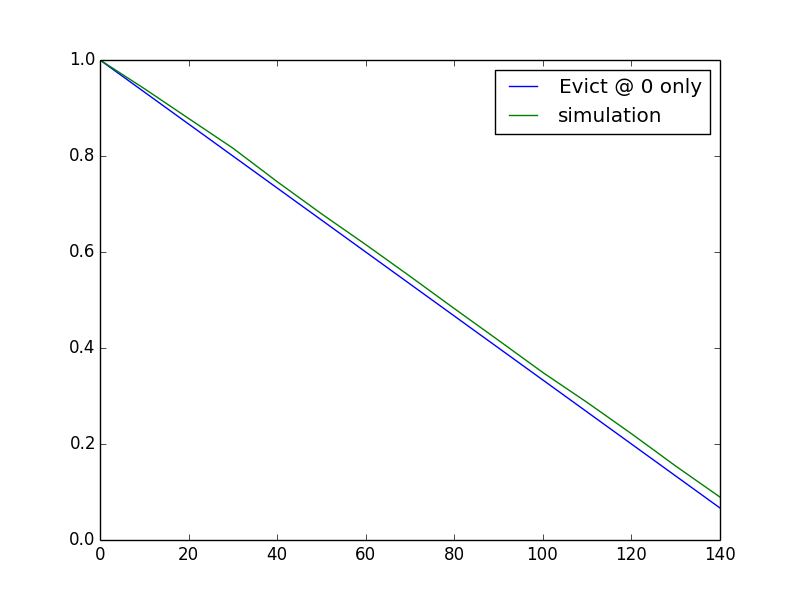
\includegraphics[width=0.5\textwidth]{sim_mru}
\caption{simulation result}
\end{figure}

\subsection{evict at d1}

\begin{figure}[H]
\centering
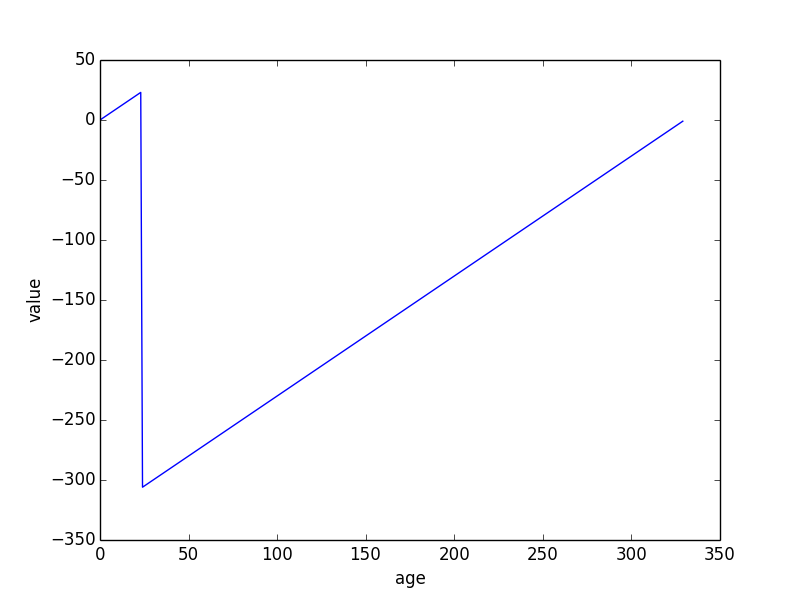
\includegraphics[width=0.5\textwidth]{evict_d1}
\caption{policy: evict candidate at age d1}
\end{figure}

\begin{table}[H]
\begin{center}
\begin{tabular}{c|c c c c}
\hline
 & 0 & d1 & d2 & d3 \\
 \hline
hit & & $p_1 x$ & \\
evict & 1-x & $(1-p_1) x$ & \\
\end{tabular}
\caption{events distribution when $0<S<d1$}
\end{center}
\end{table}

\begin{table}[H]
\begin{center}
\begin{tabular}{c | c c c c}
\hline
events & 1 & d1 & d2 & d3 \\
\hline
hit & & p1 & $\frac{p_2}{1-p_1} (1-m) $ & $\frac{p_3}{1-p_1} (1-m)$ \\
evict & & m & & \\
\hline
\end{tabular}
\caption{events distribution when $S>d_1$}
\end{center}
\end{table}

\[
m = \left\{\begin{array}{lr}
      1-p_1 \frac{S}{d_1}, & \text{for } 0 \leq S \leq d_1 \\
      (1-p_1) \frac{ed-S}{ed-d_1}, & \text{for } d_1 \leq S \leq ed
           \end{array}
           \right.
\]


\subsection{evict at d2, then 0}

\begin{figure}[H]
\centering
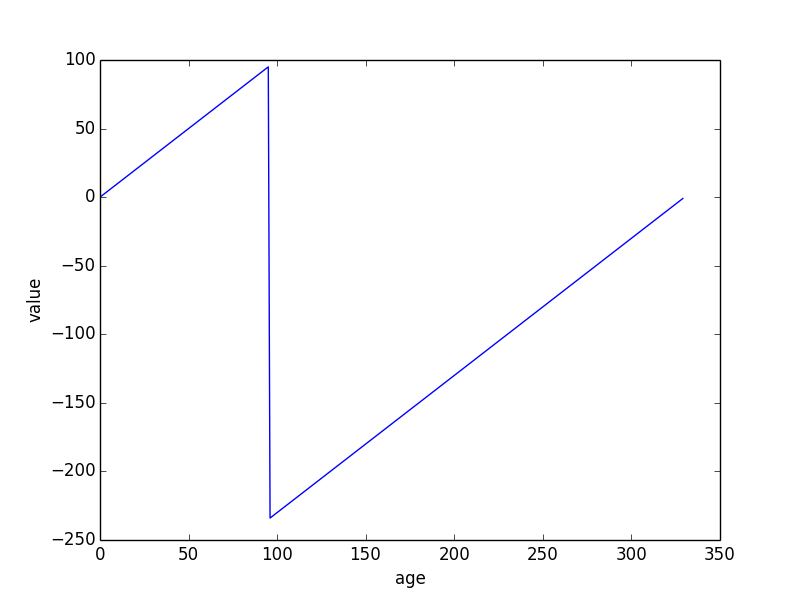
\includegraphics[width=0.5\textwidth]{evict_d2.png}
\caption{replacement policy in value function}
\end{figure}

Let x denote fraction of candidates who make it to the age of d1.

\begin{table}[H]
\begin{center}
\begin{tabular}{c | c c c c}
\hline
events & 1 & d1 & d2 & d3 \\
\hline
hit & & $p_1 x$ & $p_2 x$ &  \\
evict & 1-x & & $p_3 x$ & 
\end{tabular}
\caption{events distribution when $S<d_2$}
\end{center}
\end{table}

As cache size grow to some critical point, eviction distribution will change to
the following.

\begin{table}[H]
\begin{center}
\begin{tabular}{c | c c c c}
\hline
events & 0 & d1 & d2 & d3 \\
\hline
hit & & $p_1$ & $p_2$ & $p_3-m$ \\
evict & & & m & 
\end{tabular}
\caption{events distribution when $S > d_2$}
\end{center}
\end{table}

\[
m = \left\{\begin{array}{lr}
      1-(1-p_3) \frac{S}{p_1 d_1 + (1-p_1) d_2}, & \text{for } 0 \leq S \leq p_1*d_1 + (1-p_1)*d_1 \\
      \frac{ed-S}{d_3-d_2}, & \text{for } d_2 < S < ed
           \end{array}
           \right.
\]

\subsection{Evict at d2, d1, then 0}

\begin{figure}[H]
\centering
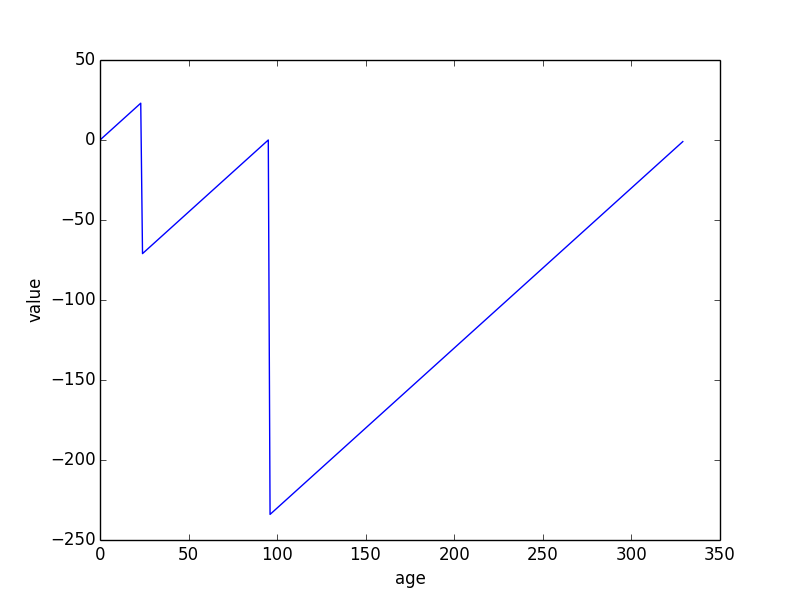
\includegraphics[width=0.5\textwidth]{evict_d2_d1.png}
\caption{replacement policy graph}
\end{figure}

Let x denote fraction of candidates who make it to the age of d1.

\begin{table}[H]
\begin{center}
\begin{tabular}{c|c c c c}
\hline
 & 0 & d1 & d2 & d3 \\
 \hline
hit & & $p_1 x$ & \\
evict & 1-x & $(1-p_1) x$ & \\
\end{tabular}
\caption{events distribution when $0<S<d1$}
\end{center}
\end{table}

\begin{table}[H]
\begin{center}
\begin{tabular}{c|c c c c}
\hline
 & 0 & d1 & d2 & d3 \\
 \hline
hit & & $p_1$ & $\frac{p_2}{1-p_1}x$ &\\
evict & & $1-x-p_1$ & $\frac{p_3}{1-p_1}x$ & \\
\end{tabular}
\caption{events distribution when $d_1<S<d_2$}
\end{center}
\end{table}

\begin{table}[H]
\begin{center}
\begin{tabular}{c|c c c c}
\hline
 & 0 & d1 & d2 & d3 \\
 \hline
hit & & $p_1$ & $p_2$ & $p_3-m$ \\
evict & & & m & \\
\end{tabular}
\caption{events distribution when $S>d_2$}
\end{center}
\end{table}

\[
m = \left\{\begin{array}{lr}
      1-p_1\frac{S}{d_1}, & \text{for } 0 < S < d_1 \\
      1-p_1-p_2\frac{S-d_1}{(1-p_1)(d_2-d_1)}, & \text{for } d_1 \leq S \leq d_2 \\
      \frac{ed-S}{d_3-d_2}, & \text{for } d_2 < S < ed
           \end{array}
           \right.
\]

\section{Solving MDP with analytical approach}

First we want to have incremental relationship in $\Delta$ space: $\Delta V_a = V_a - V_0$.

According to the value iteration update algorithm:
\begin{equation}
\begin{aligned}
V_a' = h_a (1+V_0) + e_a V_0 + l_a V_{a+1} \\
V_0' = h_0 (1+V_0) + e_0 V_0 + l_0 V_1 \\
\end{aligned}
\end{equation}

When converge, we have $V_a' - V_0' = V_a - V_0 $, that is:

\begin{equation}
\begin{aligned}
\Delta V_a & = V_a' - V_0' \\
 & = l_a \Delta V_{a+1} - l_0 \Delta V_1 + h_a - h_0
\end{aligned}
\end{equation}

Here $l_a$ denotes the leftover probability at age a, that is, $l_a = 1- h_a -
e_a$.

At smooth regions where $h_a = 0$ and $e_a = 0$, we have the slope:
\begin{equation}
\label{eq:slope}
\begin{aligned}
k & = \Delta V_{a+1} - \Delta V_a \\
& = l_0 \Delta V_1 + h_0
\end{aligned}
\end{equation}

\subsection{solving MDP in bimodal}

In bomal, the domain is $[0,d_2]$. Therefore, at age $d_2$, the modal has this property:
\begin{equation}
h_{d_2} + e_{d_2} = 1
\end{equation}

So $d_2$ is a critical point where:
\begin{equation}
\begin{aligned}
V_{d_2}' & = h_{d_2} V_0 + h_{d_2} + e_{d_2} V_0 \\
V_0' & = h_0 (1+V_0) + e_0 V_0 + l_0 V_1 \\
\Delta V_{d_2} & = V_{d_2}' - V_0' \\
& = h_{d_2} - h_0 - l_0 \Delta V_1
\end{aligned}
\end{equation}

The next critical point we look at is $d_1$, by computing $\Delta V_{d_1}$'s
value propagating from 0 and back propagating from d2, we could has another
relation between slope k and $\Delta V_1$.

\begin{equation}
\label{eq:vd1}
\begin{aligned}
\Delta V_{d_1} & = l_{d_1} \Delta V_{d_1+1} - k + h_{d_1} \\
& = \Delta V_{1} + k(d_1 - 1)
\end{aligned}
\end{equation}

\begin{equation}
\Delta V_1 + (d_1 - l_{d_1}d_1 + l_{d_1}d_2)k = 1-e_{d_1}
\end{equation}

Combining equation~\ref{eq:slope} and equation~\ref{eq:vd1}, we solve k:
\begin{equation}
\begin{aligned}
k & = \frac{l_0 (1-e_{d_1})}{1+l_0 [(h_{d_1}+e_{d_1})d_1+l_{d_1}d_2]} \\
& \approx \frac{1-e_{d_1}}{(h_{d_1}+e_{d_1})d_1+l_{d_1}d_2} \\
\end{aligned}
\end{equation}

% TODO: try to plug in different distributions based on different replacement
% policies, see if k changes.

\bibliography{main}{}
\bibliographystyle{plain}

\end{document}
